% sample.tex
\documentclass[graduation-thesis]{jsarticle}
	\usepackage[dvipdfmx]{graphicx}
	\usepackage{url}
	\usepackage{atbegshi}
	\AtBeginShipoutFirst{\special{pdf:tounicode EUC-UCS2}}
	\usepackage[dvipdfmx,setpagesize=false]{hyperref}
		\usepackage[dvipdfmx]{color}
\usepackage{url}
\usepackage{float}
\usepackage[setpagesize=false]{hyperref}
\usepackage{ascmac}
\usepackage{here}
\usepackage{txfonts}
\usepackage{listings, jlisting}
\author{61305507 情報工学科 勝又裕之}
\date{\today}
\title{}
\begin{document}


\makeatletter
\renewcommand{\thetable}{
	\thesection.\arabic{table}
} %「表(章番号)-#.」と表記するための措置
\@addtoreset{table}{section}

\renewcommand{\thefigure}{
	\thesection.\arabic{figure}
}
\@addtoreset{figure}{section} %「図(章番号)-#.」と表記するための措置

\setcounter{page}{1}

\pagenumbering{roman}
\tableofcontents
\clearpage

\pagenumbering{arabic}

\definecolor{keywords}{RGB}{255,0,90}
\definecolor{comments}{RGB}{0,0,113}
\definecolor{red}{RGB}{160,0,0}
\definecolor{green}{RGB}{0,150,0}
\lstset{
	basicstyle=\ttfamily\footnotesize,
	frame=single,
	keywordstyle=\color{keywords},
	commentstyle=\color{comments},
	stringstyle=\color{red},
	showstringspaces=false,
	identifierstyle=\color{green},
	}

\section{はじめに}
\label{intro}
 近年,マルチテナント型のクラウドにコンテナ技術が利用されている.マルチテナント型のクラウドの例として, Amazon Web Services や Google Cloud Platform がある.こういったクラウドを管理する場合に, isolation が重要である.ここで,isolation と throttle との違いを明確にしておく.ディスクへの書き込みを 15\% に制限しているが, 30\% 必要としているプロセスと, 85\% に制限しているが 50\% しか必要としていないプロセスを実行したとする.throttle であれば,前者はディスクへの書き込みを 15\% ,後者は 50\% の割合で使う.一方, isolation では,余っている分を自由に利用できるので,後者が 50\% しか利用していないため,前者は必要としている 30\% 分を使うことができる.\\
\begin{figure}[H]
	\begin{center}
		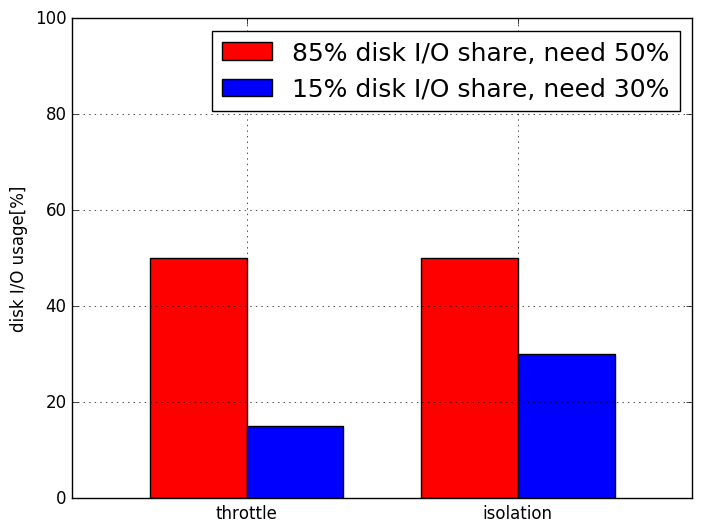
\includegraphics[width=5.0cm]{images/isolation.png}
		\caption{throttle と isolation との違い}
		\label{fig:isolation}
	\end{center}
\end{figure}
 コンテナ技術の一つとして, Linux コンテナ (LXC) がある.LXC は linux カーネル機能の一つである cgroup を利用して,コンテナ毎の資源管理を行っている.また,それによってコンテナ間の isolation を保っている.しかし, cgroup による isolation は不完全である.2個のコンテナを用意する.片方のコンテナでは cgroup によって disk I/O 使用率を 85\% に制限し,Flexible IO(FIO) write benchmark を実行する.もう一方のコンテナでは,disk I/O 使用率を 15\% に制限し,FIO write benchmark を 100 命令に一回 fsync しながら実行する.この状況では,disk I/O 使用率を 85\% に制限している方は,本来は 85\% 使えるはずが 40\% しか使えなかった.\\
 コンテナ環境における isolation の不完全性は, DDoS 攻撃への脆弱性となる可能性がある.本論文では,実際にコンテナ環境において利用される, MySQL と varmail に対して攻撃が可能であることを示し,その解析を行う.MySQL への攻撃が可能であるか検証するためコンテナを2つ用意する.片方のコンテナで, disk I/O 使用率を 85\% に制限して MySQL benchmark を実行する.もう一方のコンテナで, disk I/O 使用率を 15\% に制限して,ファイルのメタデータを頻繁に更新するスクリプトと FIO read benchmark を実行する. この時, MySQL は,本来 disk I/O を 85\% 使えるはずが,50\% しか使えていなかった.よって, MySQL に対して攻撃が可能だと言える.同様に, varmail への攻撃が可能であるか検証するためにコンテナを2つ用意する.片方のコンテナで disk I/O 使用率を 85\% に制限して varmail benchmark を実行する.もう一方のコンテナで, disk I/O 使用率を 15\% に制限して,ファイルのメタデータを頻繁に更新するスクリプトと FIO read benchmark を実行する.この時, varmail は,本来 disk I/O を 85\% 使えるはずが, 50\% しか使えていなかった.よって, varmail に対して攻撃が可能だと言える.\\
 cgroup による isolation が不完全な原因は,journal であった.LXC ではコンテナ間で file system を共有しているため,複数のコンテナの disk I/O が,一つの journal でシリアライズされる.攻撃側は,頻繁に fsync を呼び,メタデータを更新しようとしている.攻撃側の頻繁な更新リクエストにより, journal に負荷がかかる.これによって, disk I/O の遅延時間が増加するようになるが,一つの journal で管理していることによって,すべてのコンテナでこの影響を受ける.したがって,攻撃対象の遅延時間を増やし,パフォーマンスを下げることが出来たのだと考える.また,攻撃側の,メタデータの更新リクエストの頻度を上げるほど,攻撃対象の遅延時間は増加する傾向にあった.\\
 本論文の構成を以下に示す.
 第\ref{sec:LXC}章では,LXC の資源管理の仕組みについて説明する.
 第\ref{sec:journaling}章では,journaling file system の仕組みについて説明する.
 第\ref{sec:DDoS}章では,現在のコンテナ環境において, DDoS 攻撃が可能であることを示す.
 第\ref{analysis}章では, DDoS 攻撃が可能である原因を解析する.
 第\ref{relative}章では,本研究に関連する研究について紹介する.
 第\ref{conclusion}章では,まとめと今後の課題について述べる.
 
\clearpage
\section{Linux コンテナにおける資源管理}
\label{sec:LXC}
 近年,仮想化技術としてコンテナが注目されている.コンテナを実現する技術の一つに Linux コンテナ (LXC) がある.本章では, LXC の資源管理の仕組みについて説明をする.\\
 LXC は,一つのマシン上にコンテナという隔離空間を作り出す.LXC は, Linux カーネル機能の一つである cgroup を使い,コンテナへの資源の割り当てを管理している.\\
 cgroup は, OS が管理する資源を一元的に管理できる Linux カーネル機能である.cgroup は,プロセス,ファイルシステム, CPU ,メモリ, block I/O デバイスなどの各種デバイスといった多くのものを管理できる. cgroup はサブシステムによって,これら資源を管理している.
\begin{table}[htb]
	\caption{cgroup のサブシステムとその機能}
	\label{tb:subsystem}
	\begin{center}
		\begin{tabular}{|c||c|} \hline
			サブシステム名 & 機能\\
			\hline \hline
			blkio & ブロックデバイスへの入出力アクセスの制限を設定する\\
			\hline
			cpu & CPU コアの時間配分の割合を設定する\\
			\hline
			cpuacct & タスクが消費する CPU 時間をレポートする\\
			\hline
			cpuset & 使用可能な CPU コア数を設定する\\
			\hline
			devices & デバイスへのアクセスを制御する\\
			\hline
			freezer & タスクの一時停止と再開を制御する\\
			\hline
			hugetlb & cgroup からの hugetlb の使用\\
			\hline
			memory & タスクによって使用されるメモリの制限を設定する\\
			\hline
			net\_cls & プロセスが発信するパケットに識別子を付与し,制御する\\
			\hline
			net\_prio & タスクのネットワークの優先度を動的に設定する\\
			\hline
			pids & 起動するプロセス数を制限する\\
			\hline
		\end{tabular}
	\end{center}
\end{table}
 cgroup は資源のグループ化を行い,グループごとに資源利用の優先度を決めたり,利用できる資源を制限したりしている.さらに,グループを隔離することで,他のグループから中が見えないようにしている.
\begin{figure}[H]
	\begin{center}
		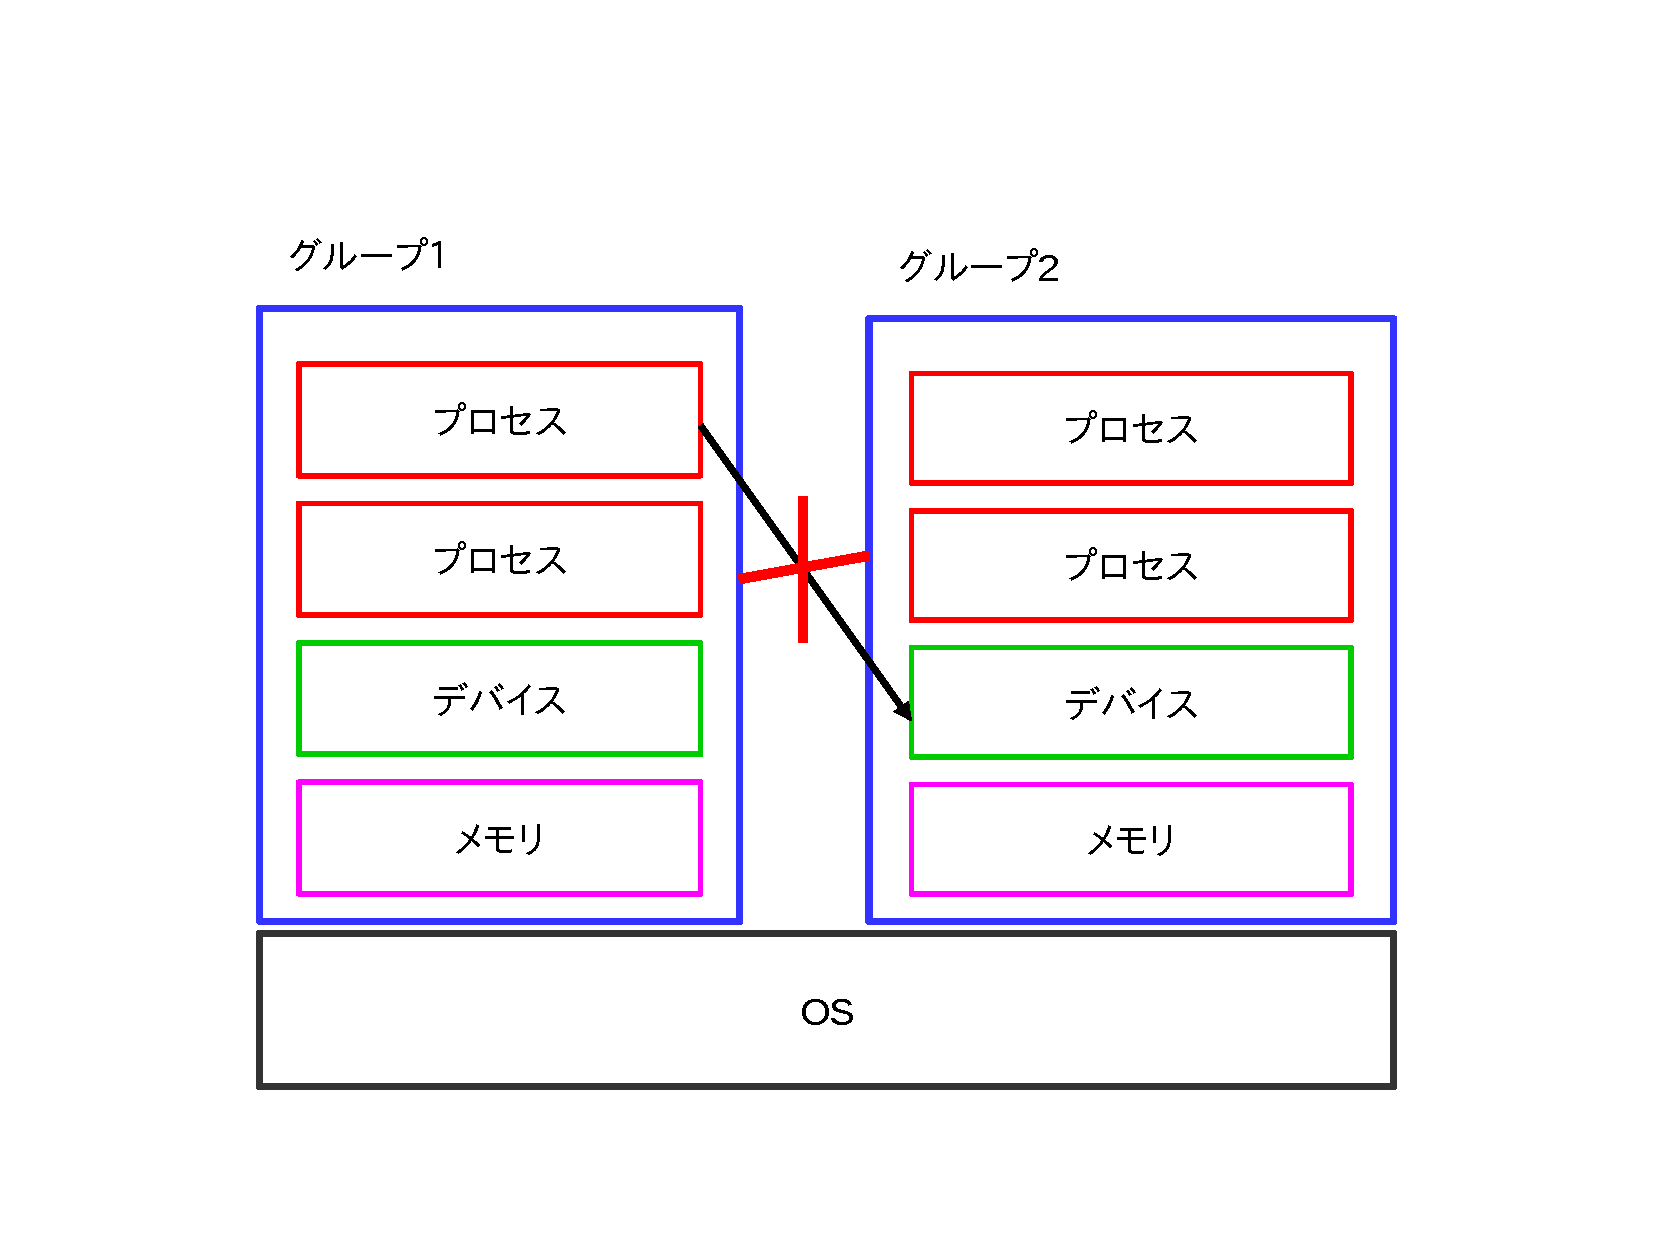
\includegraphics[width=10.0cm, clip]{images/cgroup.pdf}
		\caption{cgroup によるグループ化}
		\label{fig:grouping}
	\end{center}
\end{figure}
 
\clearpage
\section{journaling file system}
\label{sec:journaling}
\subsection{journaling の意味}
\subsection{journaling の手順}

\clearpage
\section{Linux コンテナに対する DDoS 攻撃}
\label{sec:DDoS}

\clearpage
\section{コンテナにおける資源管理の脆弱性解析}
\label{sec:analysis}

\clearpage
\section{関連研究}
\label{sec:relative}

\clearpage
\section{まとめ}
\label{sec:conclusion}

\end{document}